\documentclass[12pt]{article} % Set base font size to 12pt
\usepackage{graphicx}
\usepackage{geometry} % Adjust page margins
\usepackage{setspace} % Line spacing
\usepackage{titlesec} % Customize section titles
\usepackage{tocloft} % Customize table of contents
\usepackage{fancyhdr} % Headers and footers
\usepackage{hyperref} % Add hyperlinks
\usepackage{xcolor} % Color package

% Set page margins
\geometry{a4paper, margin=2.5cm}

% Set line spacing
\setstretch{1.5} % Adjust line spacing for better readability

% Customize section titles
\titleformat{\section}[block]{\LARGE\bfseries\color{black}}{}{0em}{\filcenter}
\titlespacing*{\section}{0pt}{3.5ex plus 1ex minus .2ex}{2.3ex plus .2ex}

% Customize table of contents
\renewcommand{\cftsecleader}{\cftdotfill{\cftdotsep}}
\renewcommand{\contentsname}{Inhaltsverzeichnis}
\renewcommand{\cftaftertoctitle}{\par\nobreak\bigskip\bigskip\bigskip} % Add space after TOC title
\setlength{\cftbeforesecskip}{0.5em} % Adjust spacing between section entries
\setlength{\cftaftertoctitleskip}{2cm} % Adjust spacing between TOC title and entries
\hypersetup{
    colorlinks=true,
    linkcolor=blue,
    filecolor=magenta,
    urlcolor=cyan,
}

% Define headers and footers
\pagestyle{fancy}
\fancyhf{} % Clear default headers and footers
\fancyhead[R]{\thepage} % Page number on right side of header
\fancyhead[L]{\nouppercase{\leftmark}} % Chapter title on left side of header
\renewcommand{\headrulewidth}{0pt} % Remove header line
\fancyfoot[C]{\thepage} % Page number in the center of footer
\renewcommand{\footrulewidth}{0pt} % Remove footer line

% Define light gray color
\definecolor{lightgray}{RGB}{240,240,240}

\begin{document}

% Title Page
\begin{titlepage}
    \centering
    \vspace*{3cm}
    {\Huge\bfseries\textcolor{blue}{\MakeUppercase{ Die geheimnisvolle Schatzsuche der Schokoladeneinhörner }}\par} % Increased font size and colored title
    \vspace{0.5cm} % Adjust space between title and author
    {\Large\textit{ Maja Schmidt }\par} % Italic author name
    \vfill
    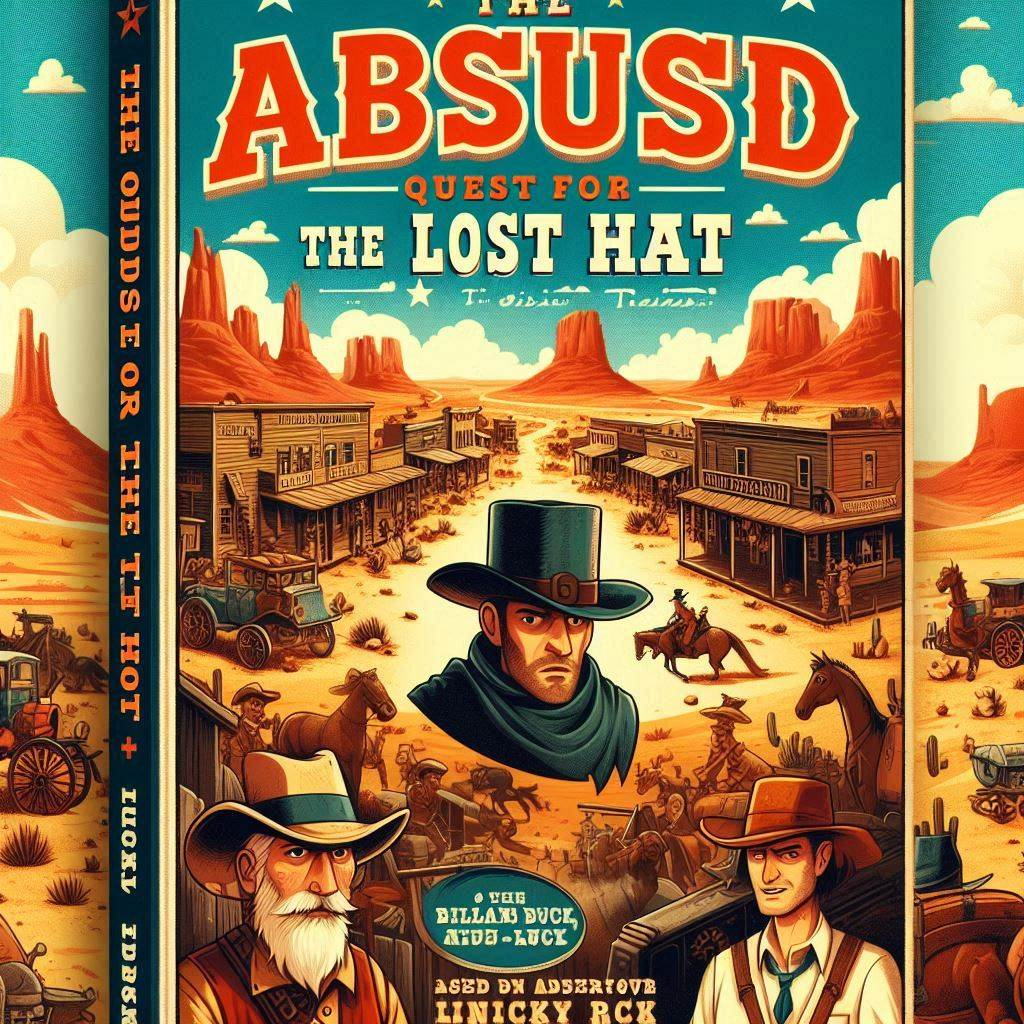
\includegraphics[width=0.9\textwidth]{ cover.jpg } % Larger cover image
    \vfill
    \today
\end{titlepage}

% Autorenvita
\section*{Autorenvita}
\vspace{4cm} % Adjust space between "Autorenvita" and "Inhaltsverzeichnis"
\begin{minipage}{\textwidth}
    Maja Schmidt ist eine erfahrene Autorin, die sich auf spannende Thriller für Kinder spezialisiert hat. Mit ihrer lebendigen und kindgerechten Schreibweise entführt sie junge Leser in aufregende Abenteuerwelten. Ihre Geschichten regen die Fantasie an und bringen Kinder zum Schmunzeln.
\end{minipage}

% Place table of contents on a separate page
\clearpage
\tableofcontents
\clearpage

% Chapters

\section{ Das Geheimnis der Schatzkarte }
\begin{minipage}{\textwidth}
    Es war ein strahlend schöner Tag im Schokoladenwald. Die Sonne schien durch die dichten Baumkronen und tauchte alles in ein warmes, goldenes Licht. Inmitten dieser zauberhaften Umgebung spielten drei mutige Kinder - Emma Einhorn, Max Schokolade und Lina Zucker. Sie waren auf der Suche nach Abenteuern und hatten keine Angst vor den Geheimnissen des Waldes. Plötzlich stieß Emma auf etwas Hartes unter einem dicken Teppich aus Schokoladenblättern. Sie hob den Teppich hoch und darunter entdeckten die Kinder eine geheimnisvolle Schatzkarte. Max rieb sich die Hände vor Aufregung und rief: 'Das ist die Karte zum verlorenen Schatz der Schokoladeneinhörner!' Die Kinder waren elektrisiert von der Vorstellung, einen echten Schatz zu finden. 'Lasst uns sofort losgehen und den Schatz suchen!' rief Lina begeistert. Und so begann ihr aufregendes Abenteuer im Schokoladenwald.
\end{minipage}

\section{ Die lustige Suche beginnt }
\begin{minipage}{\textwidth}
    Die Sonne stand hoch am Himmel, als die drei abenteuerlustigen Kinder - Emma Einhorn, Max Schokolade und Lina Zucker - sich auf den Weg durch den dichten Schokoladenwald machten. Die Bäume ragten hoch in den Himmel und warfen schokoladenfarbene Schatten auf den weichen Boden. Max führte die Gruppe mit seiner Schatzkarte an der Spitze, während Emma und Lina aufgeregt hinter ihm her liefen. 'Ich glaube, wir sind auf dem richtigen Weg', sagte Max und deutete auf eine Spur aus Schokoladenkrümeln, die sich durch den Wald schlängelte. 'Lasst uns ihnen folgen und sehen, wohin sie uns führen!' rief Emma voller Vorfreude. Die Kinder folgten der Spur und kamen an einen glitzernden Schokoladenfluss, der sich sanft durch den Wald schlängelte. 'Das muss der Schokoladenfluss sein, von dem in der Karte die Rede ist', bemerkte Lina aufgeregt. 'Aber wie kommen wir auf die andere Seite?' fragte Max nachdenklich. Plötzlich hörten sie ein leises Kichern und sahen eine Gruppe Schokoladenelfen, die auf der anderen Seite des Flusses tanzten. 'Vielleicht können uns die Schokoladenelfen helfen', schlug Lina vor. Die Kinder riefen den Elfen zu und baten um ihre Hilfe. Die Elfen, die von der fröhlichen Art der Kinder angesteckt wurden, bauten eine Schokoladenbrücke über den Fluss, damit die Kinder sicher auf die andere Seite gelangen konnten. 'Vielen Dank, liebe Elfen!' riefen die Kinder und machten sich weiter auf die Suche nach dem Schatz der Schokoladeneinhörner. Ihre abenteuerliche Reise hatte gerade erst begonnen.
\end{minipage}

\section{ Gefährliche Begegnungen im Schokoladenwald }
\begin{minipage}{\textwidth}
    Die mutigen Kinder, Emma Einhorn, Max Schokolade und Lina Zucker, setzten ihre abenteuerliche Suche im Schokoladenwald fort. Sie folgten den Hinweisen auf der geheimnisvollen Schatzkarte und wurden plötzlich von einem lauten Knistern und Knacken unterbrochen. Vor ihnen tauchte eine riesige Schokoladenstatue auf, die drohend ihre Arme ausstreckte. 'Halt! Wer wagt es, den Schokoladenwald zu betreten?' donnerte die Statue mit donnernder Stimme. Die Kinder zitterten vor Aufregung, aber Emma, die mutige Einhornjägerin, trat vor und antwortete mit fester Stimme: 'Wir sind auf der Suche nach dem verlorenen Schatz der Schokoladeneinhörner und lassen uns von dir nicht aufhalten!' Die Statue schien beeindruckt zu sein und begann zu lachen. 'Ihr seid mutig, das muss ich zugeben. Aber der Weg zum Schatz ist gefährlich und voller Prüfungen. Seid ihr bereit, euch den Herausforderungen zu stellen?' fragte die Statue. Die Kinder nickten entschlossen und die Statue öffnete einen verborgenen Pfad, der sie tiefer in den Schokoladenwald führte. Unterwegs trafen sie auf schokoladige Kreaturen, die ihre Freundschaft und ihren Mut auf die Probe stellten. Doch gemeinsam meisterten sie jede gefährliche Begegnung und kamen dem Schatz immer näher. Am Ende des Tages, als die Sonne langsam hinter den Schokoladenbergen versank, erreichten die Kinder eine geheimnisvolle Höhle, in der der Schatz der Schokoladeneinhörner verborgen sein sollte. Doch bevor sie eintreten konnten, hörten sie ein unheilvolles Knurren aus dem Dunkel der Höhle...
\end{minipage}

\section{ Rätselhafte Hinweise und knifflige Rätsel }
\begin{minipage}{\textwidth}
    Die Kinder, Emma Einhorn, Max Schokolade und Lina Zucker, standen vor einer großen Herausforderung. Sie hatten rätselhafte Hinweise entdeckt, die sie dem Schatz der Schokoladeneinhörner näherbringen sollten. Max kratzte sich nachdenklich am Kopf und sagte: 'Das ist wirklich knifflig. Aber ich bin sicher, wir können das Rätsel lösen, wenn wir zusammenarbeiten.' Emma nickte entschlossen und meinte: 'Wir dürfen keine Zeit verlieren. Die fiesen Schokoladendiebe sind uns dicht auf den Fersen.' Lina schloss die Augen und konzentrierte sich. Plötzlich begann ihr Zauberstab zu leuchten und enthüllte weitere verborgene Hinweise. 'Ich spüre die Magie des Schatzes. Lasst uns diesen Hinweisen folgen und die Rätsel lösen, um den Schatz zu finden', rief sie voller Zuversicht. Gemeinsam machten sich die Kinder auf den Weg, immer den Hinweisen folgend und dabei stets wachsam, um den fiesen Schokoladendieben zu entkommen. Doch die Rätsel wurden immer kniffliger und die Spannung stieg, als sie sich dem verborgenen Ort des Schatzes näherten.
\end{minipage}

\section{ Die fiesen Schokoladendiebe schlagen zu }
\begin{minipage}{\textwidth}
    Die Kinder hatten sich tief in den Schokoladenwald gewagt, als plötzlich ein verdächtiges Rascheln die Luft erfüllte. Max, Emma und Lina erstarrten und lauschten angestrengt. Plötzlich sprangen aus dem Dickicht drei finstere Gestalten hervor - die fiesen Schokoladendiebe! 'Halt, ihr kleinen Störenfriede! Gebt uns die Schatzkarte und wir verschonen euch vielleicht!' knurrte der Anführer der Diebe mit einem hinterhältigen Grinsen. Doch die Kinder ließen sich nicht einschüchtern. 'Den Schatz werden wir niemals herausrücken! Ihr werdet ihn nie bekommen!' rief Emma entschlossen. Ein spannender Kampf entbrannte zwischen den mutigen Kindern und den hinterhältigen Dieben. Lina nutzte ihre zauberhaften Fähigkeiten, um die Diebe mit einem Wirbel aus Zuckerstaub zu umhüllen, während Max geschickt Fallen aus Schokoladenriegeln aufstellte. Emma führte mutig den finalen Angriff an und schnappte sich die Schatzkarte zurück. Die fiesen Schokoladendiebe mussten schließlich das Feld räumen und die Kinder konnten ihre Abenteuer fortsetzen, fest entschlossen, den Schatz der Schokoladeneinhörner zu finden.
\end{minipage}

\section{ Die große Schatzsuche und ein unerwartetes Ende }
\begin{minipage}{\textwidth}
    Die Sonne strahlte über den Schokoladenbergen, als Emma Einhorn, Max Schokolade und Lina Zucker sich dem Ort näherten, an dem der verlorene Schatz der Schokoladeneinhörner versteckt sein sollte. Die Kinder hatten zahlreiche Hindernisse überwunden, gefährliche Begegnungen im Schokoladenwald gemeistert und knifflige Rätsel gelöst, um diesem Moment näher zu kommen. Als sie endlich vor der geheimnisvollen Höhle standen, die auf der Schatzkarte markiert war, spürten sie eine Mischung aus Aufregung und Nervosität. 'Das ist es, der Ort, an dem der Schatz verborgen ist', flüsterte Max mit einem breiten Grinsen. Doch plötzlich hörten sie ein unheimliches Knurren, das von tief aus der Höhle zu kommen schien. 'Was könnte das sein?' fragte Lina mit zitternder Stimme. Ohne Vorwarnung stürmten die fiesen Schokoladendiebe aus der Höhle hervor und versperrten den Kindern den Weg. 'Ihr werdet den Schatz niemals bekommen!' brüllte der Anführer der Diebe. Doch die Kinder ließen sich nicht einschüchtern. Mit Mut und Entschlossenheit stellten sie sich den Dieben entgegen. Ein spannender Kampf entbrannte, bei dem Emma ihre Einhornmagie einsetzte, Max mit seiner Cleverness die Diebe in die Irre führte und Lina mit ihrer Zuckerfeezauberkraft die Diebe in süße Träume versetzte. Schließlich gelang es den Kindern, die Diebe zu überwältigen und den Schatz zu sichern. Als sie die Höhle betraten, offenbarte sich ein atemberaubendes Schauspiel: glitzernde Schokoladenmünzen, funkelnde Edelsteine und kostbare Schätze der Schokoladeneinhörner. Die Kinder konnten ihr Glück kaum fassen. Doch plötzlich erschien eine majestätische Schokoladeneinhornkönigin und sprach zu ihnen: 'Ihr habt bewiesen, dass ihr wahre Helden seid, indem ihr den Schatz beschützt habt. Als Belohnung dürft ihr einen Wunsch äußern.' Die Kinder waren überwältigt von dieser unerwarteten Wendung. Nach einem kurzen Gespräch einigten sie sich darauf, dass ihr größter Wunsch war, dass alle Kinder der Welt die Magie des Schokoladenwaldes erleben dürfen. Die Schokoladeneinhornkönigin lächelte und gewährte ihren Wunsch. Plötzlich fühlten die Kinder, wie sich der Schokoladenwald um sie herum zu verändern begann. Die Bäume leuchteten in den schönsten Schokoladentönen, die Luft roch nach süßen Leckereien und die Kinder wussten, dass ihr Abenteuer nicht nur für sie selbst, sondern für alle Kinder ein unvergessliches Erlebnis werden würde. Und so endete die große Schatzsuche im Schokoladenwald mit einem unerwarteten Ende, das die Kinder zu wahren Helden und Botschaftern der Magie des Schokoladenwaldes machte.
\end{minipage}

\clearpage
% Metadata
\section*{Metadaten}
\begin{minipage}{\textwidth}
    \colorbox{lightgray}{
        \begin{minipage}{\dimexpr\textwidth-2\fboxsep}
            \vspace{4cm}
            \begin{itemize}
                \item Name des Buches: Die geheimnisvolle Schatzsuche der Schokoladeneinhörner
                \item Name des Autors: Maja Schmidt
                \item Name des Herausgebers: Mark Zimmermann
                \item Name des Verlags: HdM AI Technologies
                \item Adresse des Verlags: Nobelstraße 10, 70569 Stuttgart
                \item Datum der Veröffentlichung: 2022-10-20
            \end{itemize}
            \vspace{4cm}
        \end{minipage}

    }
\end{minipage}


\end{document}